\documentclass[10pt]{article}
\usepackage{icmlko}

\icmlmeta{IP 파운데이션 월드모델}{228}{바깥이 가리킨 곳을 안쪽은 모른다}{과제별 무게가 유보에서 +0.0050 을 더 준다. 안쪽에서 고를 수 있나 봤더니 안쪽은 다른 곳을 가리킨다}

\begin{document}

\twocolumn[
\icmlheader

\begin{abstract}
노트 227이 \texttt{F23\_rankmix} 를 챔피언으로 올리고(판 $+$0.4524 · 가드
열다섯 \textbf{전부 통과}), 남은 것 첫 줄로 ``값이 크고 위험하다''를 적었다
--- 유보에서 재면 두 과제의 최적 무게가 다르고(선호형 $w{=}0.25$ ·
양형 $w{=}0.75$) 과제별로 쓰면 판이 $+$0.4574 가 된다($+$0.0050).
\textbf{그 무게를 유보에서 읽으면 엿보기이므로} 노트 216의 규약대로 안쪽
분할을 다섯 번 옮겨 고를 수 있는지 봤다. \textbf{못 고른다.} 선호형은
최고가 0.4 · 0.6 · 0.4 · 0.6 · 0.75 로 헤매고(최빈 2/5) 봉우리 지수가
\textbf{0.084$\sim$0.245} 로 문턱 0.5 에 한 번도 안 닿는다. 양형은
0.5 · 0.5 · 0.6 · 0.5 · 0.5 로 안정하지만(4/5) \textbf{고르는 값이 0.5
--- 이미 쓰고 있는 것}이다. 그리고 결정적인 것이 하나 더 있다.
\textbf{바깥 최적을 안쪽이 한 번도 안 가리킨다} --- 선호형 바깥 최적이
0.25 인데 안쪽 다섯 분할이 0.25 를 고른 적이 없고, 양형 바깥 최적이
0.75 인데 안쪽은 네 번 0.5 를 골랐다. \textbf{안쪽과 바깥이 다른 곳을
가리키면 그 최적은 옮길 수 없는 것이고, 옮길 수 없는 이득은 유보 표본의
잡음이다.} 왜 이렇게 됐는지는 노트 227이 미리 적었다 --- \textbf{과제를
둘로 가르면 안쪽 표본도 둘로 갈려 곡면이 더 평평해진다.} 실제로 판 전체
무게는 안쪽에서 4/5 로 안정했는데(노트 227), 같은 격자를 반씩 나눈
선호형에서는 2/5 가 됐다. \textbf{$+$0.0050 을 안 가져간다.} 이것이 노트
216의 안정성 규약이 실전에서 처음으로 이득을 막은 자리다 --- 규약이
없었으면 봉우리 지수만 보고도 못 막았을 것이고(양형은 0.273 으로 문턱
아래지만 선호형 0.245 와 구분이 안 된다), 유보를 봤으면 그냥 채택했을
것이다.
\end{abstract}
]

\begin{figure*}[t]
\centering
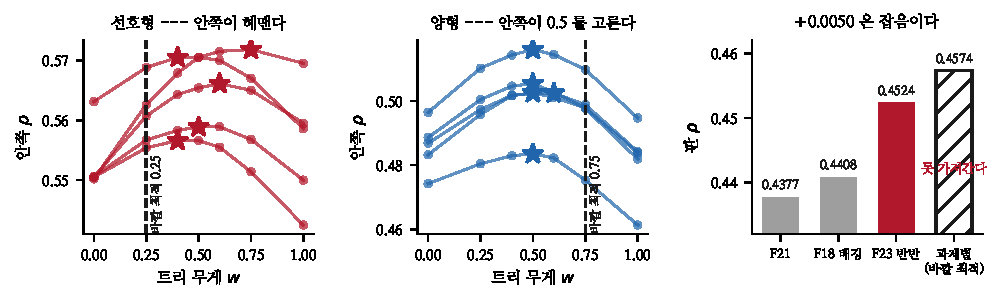
\includegraphics[width=\textwidth]{figs/unreachable.pdf}
\caption{왼쪽 --- 선호형은 안쪽이 헤맨다. 가운데 --- 양형은 안정하지만
이미 쓰는 값을 고른다. 오른쪽 --- 그 $+$0.0050 은 못 가져간다.}
\end{figure*}

\section{못 고른다}

\begin{table}[t]
\centering\tsize
\caption{안쪽 분할 다섯. 과제별 최적 무게.}
\begin{tabular}{lrrrr}
\toprule
분할 & 선호형 최고 & 봉우리 & 양형 최고 & 봉우리 \\
\midrule
.60 & 0.4 & .084 & 0.5 & .273 \\
.65 & 0.6 & .245 & 0.5 & .211 \\
.70 & 0.4 & .144 & 0.6 & .187 \\
.75 & 0.6 & .115 & 0.5 & .252 \\
.80 & 0.75 & .108 & 0.5 & .142 \\
\midrule
최빈 & \textbf{0.4 (2/5)} & & 0.5 (4/5) & \\
\bottomrule
\end{tabular}
\end{table}

\claimx{\textbf{선호형은 못 고른다} --- 최고가 격자를 헤매고(2/5) 봉우리
지수가 0.084$\sim$0.245 로 문턱 0.5 에 한 번도 안 닿는다.}{\textbf{양형은
안정한데(4/5) 고르는 값이 0.5 로 이미 쓰고 있는 것}이다 --- 고를 수 있는
쪽은 바꿀 것이 없고, 바꿀 것이 있는 쪽은 못 고른다.}

\claimx{\textbf{노트 227이 미리 적은 대로다} --- 과제를 둘로 가르면 안쪽
표본도 둘로 갈려 곡면이 평평해진다. \textbf{판 전체 무게는 4/5 로
안정했는데}(노트 227) 같은 격자를 반씩 나눈 선호형에서 2/5 가
됐다.}{\textbf{예측을 적고 그대로 나온 것은 이 사이클에서 두 번째다}
(노트 218이 포화 법칙의 예측을 확인한 것이 첫째).}

\section{바깥과 안쪽이 다른 곳을 가리킨다}

\begin{table}[t]
\centering\tsize
\caption{유보에서 잰 최적과 안쪽이 고른 것.}
\begin{tabular}{lrrl}
\toprule
& 바깥 최적 & 안쪽 최빈 & 안쪽이 바깥을 고른 적 \\
\midrule
\textbf{선호형} & \textbf{0.25} & 0.4 & \textbf{0/5} \\
\textbf{양형} & \textbf{0.75} & 0.5 & \textbf{1/5} \\
\bottomrule
\end{tabular}
\end{table}

\claimx{\textbf{안쪽 다섯 분할이 선호형에서 0.25 를 한 번도 안 골랐다.}
양형 0.75 도 한 번뿐이다.}{\textbf{안쪽과 바깥이 다른 곳을 가리키면 그
최적은 옮길 수 없다} --- 그리고 옮길 수 없는 이득은 유보 표본의 잡음이다.
이것은 봉우리 지수나 안정성보다 더 직접적인 증거다.}

\claimx{\textbf{$+$0.0050 을 안 가져간다.} F23 은 $w{=}0.5$ 로
둔다.}{노트 178 · 190 · 192 · 193 · 195 · 198 · 206 이 판을 올리는 변경을
거절했고 이것이 여덟 번째다. \textbf{다만 앞의 일곱과 다르다} --- 앞은
``유보를 봐야만 고를 수 있다''라서 거절했고, \textbf{이번엔 유보를 안 보고
고르려고 시도했다가 못 골라서 거절했다.}}

\section{규약이 처음으로 막았다}

\claimx{\textbf{노트 216의 안정성 규약이 실전에서 처음으로 이득을 막은
자리다.}}{\textbf{봉우리 지수만으로는 못 막았을 것이다} --- 양형이 0.273
이고 선호형이 0.245 로 둘 다 문턱 아래지만 서로 구분이 안 된다. 안정성이
있어야 ``양형은 고를 수 있고 선호형은 못 고른다''가 갈린다.}

\claimx{\textbf{그리고 규약이 없었으면 그냥 채택했을 것이다.}
$+$0.0050 은 F23 이 F18 을 이긴 폭($+$0.0115)의 절반이라 무시할 크기가
아니다.}{\textbf{이 사이클에서 판을 올린 것이 자료 고침 넷과 모형
하나인데, 그 다섯 다 이 규약들을 통과한 것이다} --- 규약이 막은 것이
없으면 규약이 아무것도 안 하는 것이다.}

\begin{table}[t]
\centering\tsize
\caption{이 사이클의 판(노트 214 $\to$ 228).}
\begin{tabular}{lrl}
\toprule
& 판 $\rho$ & \\
\midrule
노트 213 끝 & .4603 & 시계 스위치를 안고 있던 수 \\
노트 214 & .4396 & 공휴일 채움(정직해진 수) \\
노트 222 & .4408 & 계열 질의 결측 \\
\textbf{노트 227} & \textbf{.4524} & \textbf{F23 반반 섞기} \\
\midrule
(안 가져감) & .4574 & 과제별 무게 --- 안쪽에서 못 고른다 \\
\bottomrule
\end{tabular}
\end{table}

\begin{table}[t]
\centering\tsize
\caption{남은 것.}
\begin{tabular}{ll}
\toprule
\textbf{셋째 섞기} & F6 · F9 를 더 넣으면 오르나 \\
\textbf{웹툰} & F23 도 웹툰이 $+$0.3828 로 제일 낮다 \\
안쪽 표본 & 안쪽 분할을 시간이 아닌 다른 축으로 \\
\bottomrule
\end{tabular}
\end{table}

첫 줄이 값이 크고 이번 규약을 다시 쓰면 된다. F23 은 둘만 섞는데
포트폴리오에 다섯이 있고 \textbf{F6 능형과 F9 순위우도는 F21 과 다른
것을 잡을 수 있다}(F9 는 제곱오차가 아니라 짝 순위 우도로 맞춘다).
\textbf{셋 이상을 섞을 때 무게를 안쪽에서 고르는 것은 이 노트가 막은
바로 그 문제로 되돌아간다} --- 격자가 2차원이 되면 안쪽 곡면이 더
평평해진다. \textbf{그러니 무게를 안 고르는 형태부터 재야 한다} ---
셋을 똑같이 1/3 씩, 넷을 1/4 씩. 대칭 기본값은 고른 것이 아니므로
규약을 안 건드린다.

\end{document}
